\chapter{Discussion and Future Work}
\label{Discussion}

\section{Introduction}
\label{Discussion:Intro}

In this thesis, I have explored the experiences and perspectives of stakeholders commonly implicated in design processes in designing with and for people with dementia, with the aim of broadening the conversation surrounding technology design with and for people with dementia. This thesis argues that while there has been a breadth of literature on involving people with dementia in technology design processes, research has often overlooked the needs and interests of stakeholders commonly implicated in design processes. For instance, through this thesis, I worked closely with family members, designers, developers, and researchers as well as people with dementia which in turn, has developed a more relational perspective of the design process for people with dementia.

Through reviewing the literature, I report on the role of co-design and participation in dementia and HCI, emphasising the need to accommodate the different needs of people with dementia, ensuring they are respected rather than infantilised. Furthermore, to support collaboration and engagement between those who are being designed for and those who are designing, I present four areas of investigation that are associated with the four data chapters: 
\begin{itemize}
    \item Attending to mutual collaborative relationships
    \item Representation of technology and dementia from a designer/developer perspective
    \item Ethical practice in dementia-HCI
    \item Promoting learning around dementia and technology
\end{itemize}

In chapter four, I introduce a reflective account of two studies working with families and individuals living with dementia. In these studies, I explored the opportunities and challenges of designing personalised media experiences that considers an individual's history, interests, personality, desires, and ecology of care \citep{ryan_dementia_2009}. The first study explores designing tailored VR environments for people with dementia that places emphasis on reminiscence and the second study, explores media capture of meaningful experiences to support families living with dementia that questions whether approaches that rely on the person's ability to recognise or articulate past events is an appropriate activity to enhance emotional connection. I conclude this chapter by outlining the ethical challenges of building technology for different needs and interests. As I describe in this chapter, engaging with people with dementia required a long-term process of upskilling myself to conduct sensitive and ethical research appropriately. However, at the time, the VR work was gaining local authorities' interest, resulting in a hackathon event. This provided the opportunity to unpack how you might design a public-facing event to suitably teach and create a safe space for learning about dementia and VR.

In chapter five, I explore public engagement with the topic of dementia. I ran a two-day hackathon called DemVR, which aimed to provide a space for participants to design novel use cases of shared VR experiences for people with dementia and care partners. Much HCI and dementia research describe the importance of sensitive design to support close and personal interactions. However, the approach often requires long-term engagement between researchers and participants that are often not doable for many design processes such as design sprints due to the fast nature of the approach \citep{braybrooke2021care}. In this chapter, I revisit the hackathon structure to reflect on how the event's design led to a lack of involvement of people with dementia and care partners. The analysis presents insights into participants' motivations, challenges participants faced when constructing their `absent user', and the design features teams developed to address the user's social context. I conclude the chapter with a set of commitments that offer insights into how we might mitigate stereotypes in constructing the end-user; ways to improve recruitment for marginalised populations in events; and steps to promote more inclusive, community-driven events. Chapters four and five describe the ethical challenges when working in sensitive settings and the knock-on effects that occur to design ideas when the end-user is not involved in the design process. Given that many papers reflect on participation in dementia and HCI, the following chapter takes design ethics in dementia and HCI to reflect as a community of practice.

In response, chapter six invites 22 researchers from dementia and HCI practice to come together to elucidate broader concerns about ethics in HCI research. In chapter six, I provide an understanding of ethical concerns stemming from diverse countries, institutions, and disciplines. The findings uncover tensions arising from institutional ethical practices in socially oriented research. Through the interviews, researchers argued how ERBs could act as reflexive bodies where researchers can seek support, guidance, and collaboration from and with experts. Researchers also shared insights from their cultivated practices: establishing clear expectations for participants, knowing when and how to involve participants in the research, and appropriately acknowledging their contributions to our work. I proceed from the findings to emphasise directions applicable in all HCI research that seeks to work with marginalised populations: suggestions to improve the relationship between researchers and ERBs, re-framing impact and the shift towards peer-led research. Following the three chapters, a recurring theme in the findings was how collaboration could be engaging and meaningful between people with dementia and stakeholders commonly implicated in design processes.

Aware of the challenges of involving and designing for people with dementia, particularly for those with little to no training, chapter seven explores design activities that evoke creativity and learning for designers and developers. This study recruited seven designers, four developers, and five people with dementia, to participate in a three-stage iterative process to explore the type of resources developers and designers need to design with people with dementia and investigate how people with dementia envision their potential participation within a toolkit. Following stages one and two, I used a process of affinity diagramming to help surface a set of design priorities to guide our design for a final dementia design toolkit prototype – which I call the Dialogical Dementia Design (D3) Toolkit. Within this toolkit, I provide several activities to provide designers/developers with an ethical and sensitive way to engage with people with dementia, critically think about relevant aspects of dementia, and curate toolkit resources to be community-driven through the inclusion of varying stakeholders’ involvement. Following the toolkit design, I conducted a workshop to reflect on the prototype toolkit to provide insights into how designers, developers and people with dementia may contribute, use, and envisage how toolkit components might facilitate co-creation between different groups.

In the remainder of this chapter, I revisit the main research aim :
\begin{quote}
\textbf{\textit{``How might participation be configured for people with dementia to shape the design process of technology''}}
\end{quote}

The subsection below explores the lessons learned across the data chapters and is split into the three research questions I set out at the start of the thesis. After reviewing the research questions, I describe a proposed approach for future work. In this future work, I reimagine the role of participation between people with dementia and diverse stakeholders to move towards a more inclusive design space that supports mutuality in the co-creation of new technologies and systems. 

\section{Participatory approaches}
\label{Discussion:RQ1}
\begin{quote}
\textbf{    Research Question 1:
}    
\textit{    “How can we use participatory design approaches to provide meaningful and engaging experiences for people with dementia?”}
\end{quote}

Across the thesis, I worked with multiple people with dementia and care partners who come from various backgrounds and stages of dementia. To answer the question regarding ways to provide engaging and meaningful participation for people with dementia, this section describes the importance of recruitment techniques, and adapting participatory methods to ensure people with dementia are involved and can contribute to the design of technology. 

\subsubsection{Recruitment techniques}
\label{RecruitmentTechniques}
During the thesis, participation and recruitment has been tackled in many ways resulting in a variety of challenges and opportunities. For instance, in chapter four, I worked closely with Silverline Memories, which supported members' interest in partaking in the study. Working closely with Sandra at Silverline provided information about any requirements the person with dementia might need to participate. However, this heavily relied on the organisations participation and assistance in recruiting members that they felt would be best suited for the research. \cite{kristensen2015voices} states that recruitment presents several implications that impact knowledge production. For instance, working with Silverline Memories limited the selection criteria for participants because Sandra picked the families she felt would be more engaged in participating. Although this helped to make the process relatively straightforward, working with families who may have been less interested in VR may have resulted in significantly different findings.

Furthermore, in chapter seven, I asked participants if they needed or had any expectations from the study to improve their participation. This ranged from sending overview emails of the interviews; 15-minute reminders before the meeting; and a breakdown of all the quotes I would use from their interviews in the PhD. In chapter five, recruiting people with dementia and care partners to join the online platform for DemVR was a challenge. As the chapter states, people with dementia had little to no interest in participating or using the online platform. In contrast, \cite{namageyo2014recruitment} stresses the impact that interview or workshop locations have on recruitment. The authors report that \textit{``participants are less likely to enroll in a research study if the location is not convenient''}. Similarly, in chapter four, the families chose locations to partake in the research, providing a safe space for sharing stories. When it comes to participating online, researchers should expect the same.  

Instead of designing additional online platforms, I suggest asking participants what platforms they would like to use for engagement. Not only does this reduce development costs, but this also provides the opportunity to understand the communication processes with which participants are familiar. One approach I might have adopted would be an ‘Unplatformed’ approach to the design of the pre-hackathon experience and recruitment stage. Unplatformed design is a model for the appropriation of social media technologies, that pays particular attention to the implications of the individual features of social media in respect to coordinating participation in specific contexts \citep{lambton-howard_unplatformed_2020}. I might have reduced barriers to engagement and ensured better representation of the views of the participants by coordinating participation on the technologies that they were already comfortable with (e.g., Twitter, Facebook, and other media platforms). 

However, it should also be noted that utilising solely digital methods to facilitate recruitment and engagement could be limiting for some participants facing significant marginalisation. For instance, \cite{lazar_safe_2019} describe how even inclusive initiatives centred around the involvement of people with dementia may silence voices that offer less \textit{``polished stories''} or those who are nonverbal. \cite{dai2020making} describe that while online interactions provide an enjoyable and beneficial interaction for the person with dementia, it contributes to a burden and the need for the care partner to provide \textit{``responsive, continuous, and knowledgeable support'' }\citep[pg. 46:24]{hwang2020exploring}. Moreover, we should consider ways to invite and involve not only people with dementia, but their care partners, friends, and family in the research process to help ensure agendas are more closely aligned with stakeholders’ priorities and desires. To this extent, participant-led research may offer understandings into new, more impactful ways our research could benefit communities beyond academic publications.

\subsection{Adapting participatory methods}
\label{AdoptingMethods}
Within the methodology chapter, I reported that HCI researchers adapt traditional research approaches to make their methods flexible and tailored to the needs of people with dementia \citep{webb2020misfitting}. In chapter four, where I worked closely with families with dementia, I adapted traditional interviews into `walking interviews' \citep{kullberg2017walking} where families went on a day out. While the literature highlights that specific methods such as workshops and interviews are more suited for people in the early stages of dementia \citep{lindsay_empathy_2012}, given that the participants with dementia were rarely verbal, the walking interviews helped to capture more embodied interactions where their contributions could be more observation. For instance, Sarah would occasionally pull bark off a tree and encourage me to hold it, or Lauren grabbing my arm to direct me towards flowers or a family of ducks across the Chinese Pond. This approach did not limit the people with dementia as it was not necessary for participants to require to rely on their memory or recall abilities to contribute to the study. By adopting such an approach, I spent a lot of time getting to know the families outside of the study space to ensure that I built trust and a relationship with the participants. 

While building rapport with the families helped to understand how they might use the media experiences, in chapter six where I interviewed HCI researchers, Lucas iterated how the longer-term projects can have knock-on effects. For example, while he agrees that longer-term projects are necessary to build relationships with participants, during the iteration design phase, the prototype or system should be changing frequently to show the participants that their feedback is being recognised and is shaping the design. These insights offer questions concerning how much time is spend building relationships compared to demonstrating the iterative design and development process.

Additionally, in chapter seven, dementia advocates explained their uncertainty of how their insights would be used. Howard and Masood wanted to see what quotes I would be using in the PhD to ensure if any of them would be \textit{``out of context''}. To validate my findings, I fed back the analysis and findings to those who were interested to check if my interpretation was accurate. This process is a popular approach known as `respondent validation' \citep{richards2002ethics}. However, although I was able to provide Howard and Masood with the reassurance how their data was being used, they both shared concern that this is difficult when they consult and share their experiences to organisation.

In this PhD, I have attempted to document the different ways I have adapted my participatory methods to demonstrate what was required. In this way, chapter six, where I invited 22 HCI researchers to describe their experiences with working in HCI in the context of dementia, the findings attempt to document the challenges and processes HCI researchers have put in place to recognise and ensure the person with dementia participates and contributes to the design of technology. For future work, researchers must continue to publish better documentation of their processes to ensure developers, designers, and researchers can build on top of an already growing practitioner base.

\subsection{Summary}
\label{RQ1:Summary}
Ultimately, although people with dementia can participate in engaging ways, the process requires thorough consideration by the researcher to ensure people with dementia are respected, listened and recruited in a way that works for them. As such, through exploring this research question, the thesis provides the following insights:

\begin{itemize}
    \item Work closely with stakeholders to ensure you can flexibly accommodate their needs for engaging in technology design.
    \item For later stages of dementia, or those who might not be verbal, participatory methods require more creative processes that move away from traditional methods such as interviews and workshops. This might require care partners or friends enacting in a supportive role.
    \item For recruitment and participation, researchers should consider the needs and interests of care partners and organisations acting as gatekeepers. This should also extend to engagement online whether that is recruiting through platforms, or research engagement through social media platforms. 
\end{itemize}

\section{Ethical implications in dementia and HCI}
\label{Discussion:RQ2}
\begin{quote}
\textbf{    Research Question 2:
}    
\textit{    “What are the ethical implications for people with dementia to participate in HCI research?”}
\end{quote}

Across the thesis, I have examined various ethical challenges underpinning research in the area of dementia and HCI. In many of the examples in this thesis, ethical challenges involving people with dementia stemmed from attaining consent and researching under a culture of ethical 'protectionism'. To answer the research question, I have split this section into the following: a) implications for attaining consent; b)  building community understanding for ERBs; and c) involving those further under-represented in dementia.

\subsection{Implications for consent}
\label{Cosent-Implications}
In chapter six, many of the researchers stressed the tendency for ethical review boards (ERBs) to see people with dementia as 'vulnerable'. \cite{pachana_can_2014} further highlights that committees may be \textit{``subject to the same biases and stereotypes present in the general population''}. ERBs that are unaware of such biases, may focus on the aims of protection, as opposed to the approval of research that attends to topics such as agency and ensure meaningful participation. For instance, as I describe in chapter four, Philip could not provide informed consent to participate at the given moment. In accordance to the Mental Capacity Act (2005):

\begin{quote}
\textit{``A person lacks capacity in relation to a matter if at the material time he is unable to make a decision for himself in relation to the matter because of an impairment of, or a disturbance in the functioning of, the mind or brain.''} \citep{oyebode_mental_2005}
\end{quote}

As demonstrated in chapter four, Philip's ability to make decisions seemed to fluctuate depending on the time of day, and interactions throughout the day. However, that might suggest that the consent procedure should be taken when the person with dementia is having a 'better day' than other days, which still restricts a very ambiguous process and requires flexibility \citep{trachsel2015cognitive}. 

\cite{o2021advocating} argue that \textit{``although a person with dementia may have been deemed to lack capacity to make complex life decisions, it does not necessarily follow that they will not have capacity to understand the general nature and activities of a study''}. \cite{dewing_participatory_2007} describes a process of consent that centres on the individual's values and interests. Through this process, Dewing suggests that those who cannot legally formally consent can still engage through 'inclusionary consent' based on experiential preferences that come from building researcher-participant relationships. Further, Dewing stresses that the consent process should continue through the research process. Future work in dementia-HCI must consider how researchers can ensure consent without limiting the participation and contribution of the participant. 

\subsection{Connecting ERBs with community members}
\label{ERBs-Community-Members}
In chapter six, researchers raised a range of concerns with ERBs when the ERB does not have the insight into the topic at hand. As several researchers report, this may result in the committee that see dementia in a biomedical perspective causing conflict in the judgement of what people with dementia can and cannot do. One option would be for researchers to provide training support to committee members on the topics of dementia. For instance, \cite{goldberg2015relationship} reviews a dementia-focused Massive Open Online Course (MOOC), demonstrating a significant reduction in stereotypical assumptions on the capabilities of people with dementia. However, adopting such an approach would require committee members to take courses and training for other non-expert topics, which would not be possible given how many topics ERBs have to consider. 

Alternatively, \cite{lidz2012participation} reports on community members' participation on a medical institutional review board. While the authors initially write issues regarding community members playing a lesser role than other institutional members, the authors convey that over time, community members helped provide helpful insight into consent processes, particularly on confidentiality and privacy topics. Similarly, in the thesis, I report several times where researchers suggest researchers should build tools for community members and ERBs to promote conversation and inclusion. \cite{davies2021dementia} co-authored a paper with six people with dementia that explores Dementia Enquirers, a dementia advocacy group, who are developing ethical guides and best approaches for dementia research to support the design and development of ethically designed dementia research. For researchers, we might consider how to connect advocacy groups (like Dementia Enquirers), to the University ERB committees. With Dementia Enquirers building an ethics panel and a set of ethical standards for involving people with dementia, perhaps institutional ethics might consider inviting these community-led panels to handle ethical issues and approvals on behalf of the community they represent. That way, people with dementia can provide valuable pre-design feedback and ensure research designs are rooted in community-led agendas. 

\subsection{Involving people further under-represented in dementia.}
\label{Under-represented--dementia}
Within HCI, there is increased attention to incorporating the voices of underrepresented populations to support issues of health, wellbeing and political engagement \citep{erete_intersectional_2018}. \cite{harrington_forgotten_2020} states that researchers are starting to involve groups or communities who sit at the `forgotten margins'. These margins comprise of people who are continued to be neglected by research and design efforts. For instance, these groups are people who might identify as people with dementia, but have cultural or sexual identities that further marginalise that person or group. 

From the work I conducted in the North East, the families I worked with were predominantly from a working-class background, white and in a heterosexual relationship. Given that only 11\% of Newcastle's total population are black, Asian or minority ethnic (BAME), it is no surprise that the members of Silverline Memories came from very similar upbringings and backgrounds \citep{cityCouncil_2021}. Meanwhile, in chapter seven, I worked with a number of people with dementia from mixed backgrounds, such as an accountant, human rights lawyer, and social worker. In particular, Masood originally came from Pakistan and moved to the UK as a teenager. When interviewing Masood, I became aware of several implications that might make participation challenges that had not become apparent in my prior work. For instance, Masood mentioned how much of the diagnosis content he received was in English. However, he stresses that \textit{``for others whose English is their second language, accessing [living with dementia] resources is extremely inaccessible''}. This resonates with the work by \cite{cooper2018relationship}, who writes about how non-native speakers with dementia experience agitation where no residents or care staff share the person's same language or culture. Masood continued by emphasising that linguistic and cultural barriers would contribute to his family \textit{``having a lack of understanding about dementia, who would sometimes have offensive views of dementia''}. In this way, from the interviews with Masood, I gained unique understandings that are not apparent in conversations with people at Silverline Memories. 

With this in mind, researchers might want to consider how we might invite and involve groups that are further underrepresented, such as, the LGBTQ+ community, young onset dementia, advanced dementia and people with other cultural and diverse backgrounds \citep{foley_struggle_2019, bryden_before_2015}. \cite{mcgovern2014forgotten} describes designing spaces for safety and belonging that provide people with dementia in the LGBTQ+ community to open up and share their stories. The authors suggest that to build a meaningful and safe space, researchers should accept diversity; adopt language that represents the community; and use language and images that represent the community during recruitment, whether in information sheets, marketing materials, or leaflets. Further, when talking with Howard who is a dementia advocate for 3 Nations Working Group, he mentioned that the group has \textit{``started to get people from ethnic, LGBTQ+ backgrounds, but it is still far from being done...''}. As researchers often have the unique opportunity of working with those who are under-represented, researchers should consider that part of their research impact should be to build connections between participants and dementia networks to support growth and inclusivity.

\subsection{Summary}
\label{EthicsSummary}
From this section, the main point here is that there are several infrastructures that stop research and practice from being more inclusive and meaningful. However, to move towards a practice that ensures people with dementia are valued and can participate and contribute to the extent they want to, researchers might consider the following:
\begin{itemize}
    \item Educate members of ERBs, and others, about the ramifications that a biomedical view portrays.
    \item Researchers to support and guide participants from underrepresented communities to be part of other dementia networks and advocacy groups.
    \item Tailor the consent process to the needs and requirements of the person with dementia.
\end{itemize}

\section{Supporting meaningful dialogue}
\label{Discussion:RQ3}
\begin{quote}
\textbf{    Research Question 3:
}    
\textit{ “What are the competing interests and expectations to support meaningful dialogue in dementia design research when involving multiple stakeholders - such as people with dementia, developers, designers and researchers?”}
\end{quote}

The final research question is concerned with the different interests and desires of the diverse set of stakeholders I collaborated with within the thesis. To answer the research question, I have split the section into two subsections: a) considerations for stakeholders implicated in the design process, and b) the expectations and considerations from people with dementia and care partners.

\subsection{Stakeholders implicated in the design process}
\label{DevsDesigners}
At a time when technology has become increasingly complex, adopted into our daily lives, and ubiquitous, researchers are drawing attention to the design and deployment of technology \citep{west_data_2019}. For instance, in recent years, HCI researchers have begun recognising the real-world harms that AI integration's may cause \citep{borenstein2021emerging}. In response, the AI community has worked closely with activists and advocacy groups to find ways to learn and support their work to empower communities through tools or systems for understanding data collection. One popular approach in teaching methods on accountability and transparency has been through the building of toolkits. For instance, \cite{krafft2021action} co-designed an Algorithmic Equity Toolkit that provides AI researchers reflective questions to surface the social context of the system, and activities to better understand how machine learning works and how it fails. The processes to improve the ethical design of AI resonates with \cite{mulvenna_ethical_2017} manifesto called `Ethical by Design'. The manifesto proposes several principles such as `seek to integrate with and support the progression of policy'; `Be realistic about what is possible and needed; `provide enough information for people to make informed decisions at every stage about whether, when and, and how to use the product or service'. 

In chapter seven, three of the four developers voiced that while they \textit{``know [their] designs should be more considerate and ethical,   but when they are time constraints and a limited team, there is only so much [they] can do''}. In this way, designing approaches to provide more ethical solutions in technology design requires considering how toolkits and approaches fit into the designer's or developer's workflow. In chapter five, while prize money was a contributor to encouraging participation in the weekend, multiple teams indicated pro-social motivations. For instance, Garden Life, were driven to \textit{``deepen [their] understanding of these issues''} in the hope of \textit{``alleviating the stigma'}'. Similarly, when talking about community-led projects in chapter seven, Husainah suggested how some designers may contribute because their skillset could help others. However, Husainah and other designers did say they would only contribute in small amounts where they might provide help on a weekend or evenings. 

In summary, through the thesis, designers and developers have shown a keen interest in working with people with dementia, mainly where it provides learning opportunities or the chance to help others. However, at the same time, designers and developers expressed that supporting that dialogue in the development of technology can become challenging when it collides with their workflows, even when they explicitly acknowledge the importance of involving the voices of the users they are designing for.

\subsection{People with dementia and care partners}
\label{PwDInterests}
Within dementia advocacy, a recent movement mirrors the disability rights and disability justice activists who popularised the phrase \textit{``nothing about us without us''} \citep{spiel_nothing_2020}. For example, Dementia Alliance International uses this term in their stated goal of eradicating stigma and discrimination and recognises the eligibility for anti-discriminatory disability rights for both people with dementia and their supporters \citep{oldfield2021nothing}. Through this, we have seen a rise in advocacy groups and advocates campaigning for change through blogs, keynotes, and other campaigning activities to discuss the social and individual challenges of living with dementia \citep{thomas2018dementia}.

In chapter seven, I worked closely with advocates with dementia in building a collaborative toolkit to support the design for dementia. During the interviews, people with dementia raised concerns about the lack of recognition they get when participating in design processes. In one instance, Masood described frustrations of \textit{``feel[ing] like a guinea pigs''} where he would never hear from the researcher once they had all the information they needed. Similarly, the participants said they are often `giving' away their experiences and expert knowledge for free. \cite{wiersma2016creating} interviewed dementia advocates who reported a psycho-emotional burden where the public would comment on how the person is a fraud as their dementia does not represent the current public perception. Through the thesis, people with dementia have reported wanting to be part of the participatory process and design alongside other stakeholders. However, when treated as unequal and not recognised for their contribution, participants described disinterest and exhaustion of their continued work as advocates. 

In contrast, in chapter four, while the families were interested in the design process of the moment boxes, the interest in partaking in the study came from choosing where to go on a day-out. Given that some family members were rarely verbal, I sought value in involving the ecology of care around the person with dementia. In doing so, the chapter provides insights into ways to manage conflicting expectations between the person with dementia and their care partner. Furthermore, the chapter recognises that with many carers reporting high levels of burnout and burden \citep{lee_technology-based_2015},  targeting carers as research participants worthy of digital interventions focusing on personhood (as much as we target those with dementia) means treating them with respect, and as whole persons, rather than defining them by their roles. 

As previously mentioned in chapter five, although the hackathon was centred on shared experiences for people with dementia, the topic lacked any primary focus on care partners, families, and friends – those who make up the ecology of care for the person with dementia. In hindsight, undermining care partners desires and interests may have contributed to the struggle in recruitment. When looking back at the hackathon, teams' ideas that emphasised care partners typically came from facilitators' feedback instead of the introductory presentations or Howard's Q\&A. For instance, Chatter Bench describes a facilitator as \textit{``opening up their eyes''} to the potential burden to care staff if the technology requires significant assistance. 

Moreover, \citeauthor{dai2020making}'s work into a community-based social group for people with dementia presents the complexities care partners have in mediating social cues and communication for the person with dementia when engaging online \citep{dai2020making}. The authors draw attention to the strain and potential ``burdening" that this can cause, despite the benefits of people with dementia sharing their experiences and partaking in activities. Here, researchers must consider how they can design tools and methods to promote conversation and include the voices of a diverse set of stakeholders to ensure we are designing technologies that pay attention to both the desires and interests of the person with dementia and their ecology of care.

\subsubsection{Summary}
\label{RQ3-summary}
Through working with people with dementia, care partners and stakeholders implicated in the design process, I have examined a series of expectations and interests that researchers might consider to support meaningful dialogue between the different stakeholders. To summarise the response to the research question, I  suggest the following:
\begin{itemize}
    \item Acknowledge the stakeholder's contribution through finding appropriate incentives - whether this is learning more about an area, or being paid for their expert knowledge.
    \item Given the complex and necessary support people with dementia might need from care partners, care staff or volunteers, researchers should involve the ecology of care in the research agenda. Furthermore, their involvement should move beyond using care partners as solely communicative tools for understanding the person with dementia's interests and desires. Instead, they should be treated as whole persons rather than defined by their caring role.
    \item While designers and developers acknowledge the importance of ethical design and involving the voices of the people they are designing for, often co-design and participatory approaches do not fit into the designer/developer's existing workflow.

\end{itemize}




\section{Future work: Balancing stakeholder interest}
\label{Discussion:Design}

\begin{figure}[htp]
\centering
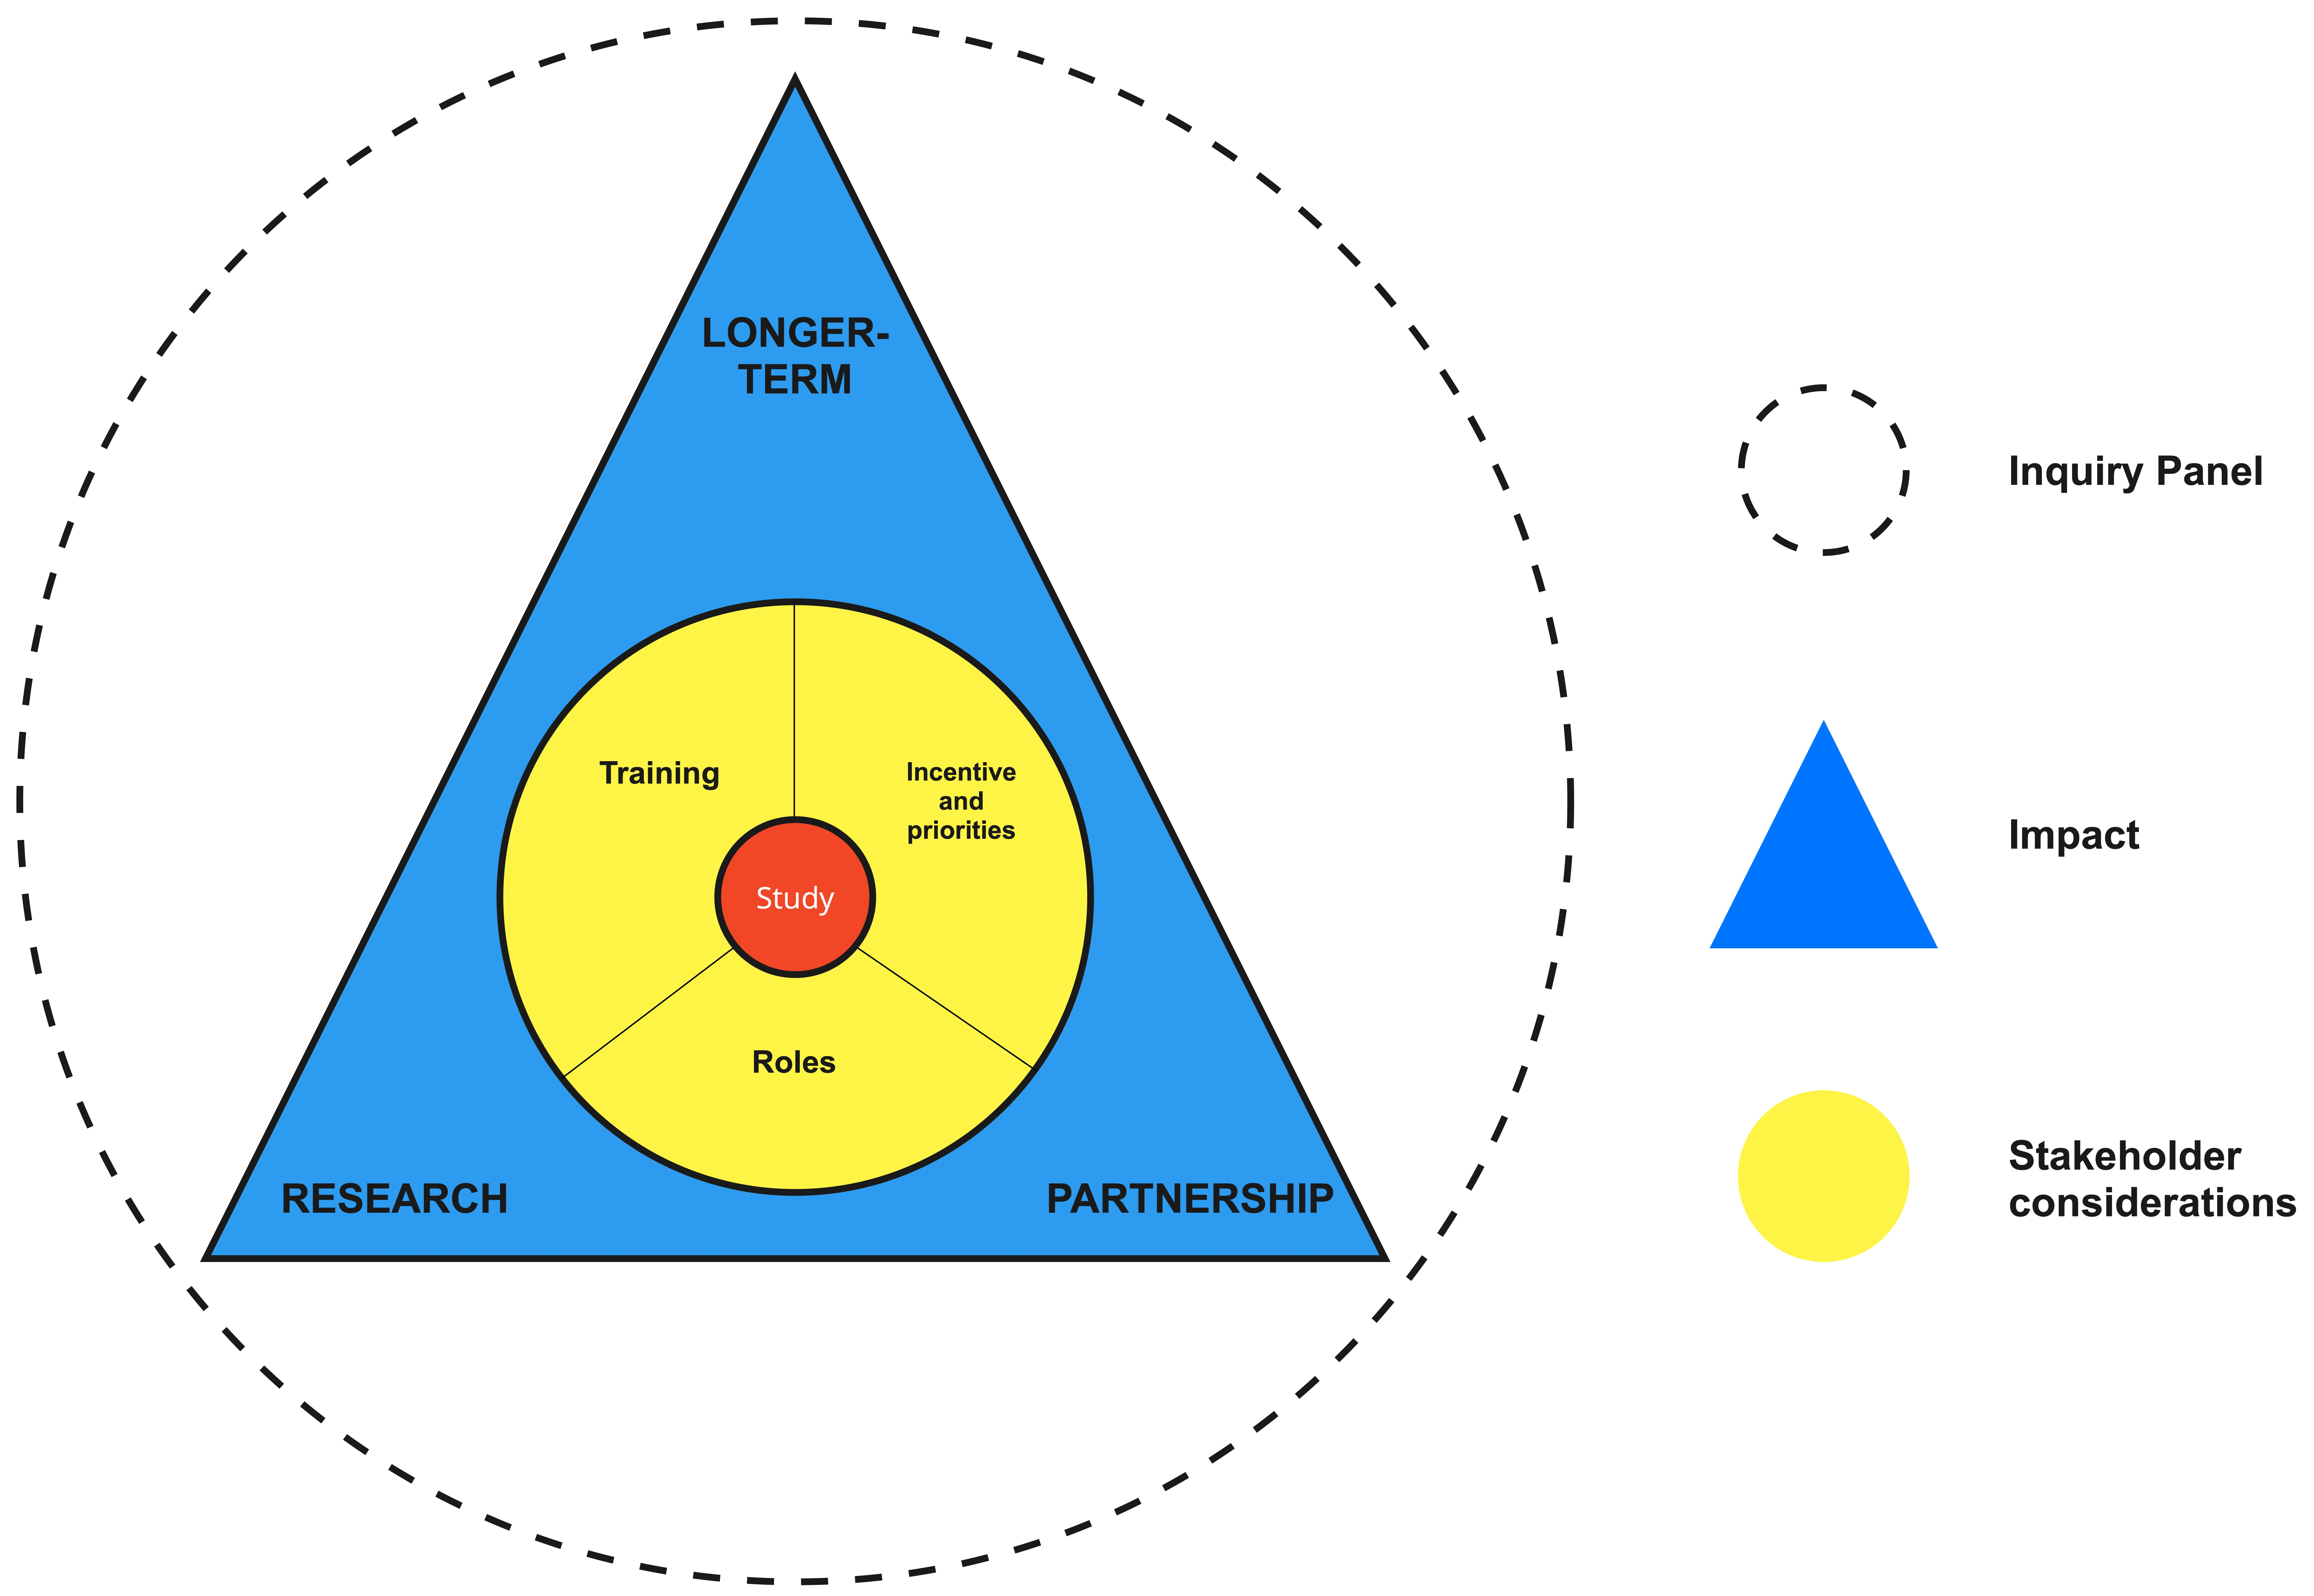
\includegraphics[width=0.8\linewidth]{Images/Discussion/DesignApproach.jpg}
\caption{Balancing stakeholder interest diagram}
\label{fig:MeaningfulParticipation}
\end{figure}
To suggest future work in HCI in the context of dementia, I propose a set of components to \textit{balance stakeholder interest}. The approach draws on the insights from the previous data chapters to provide ways to engage and broaden the dementia debate through a more inclusive approach. The approach consists of three core components that surround a research study. By considering the three components, the aim is for researchers to critically reflect and consider ways to improve stakeholder engagement, ethically engage with research impact, and ensure research designs are rooted in participant-led agendas. The three components are the following:

\begin{itemize}
    \item \textbf{Inquiry Panel}: Developing a group of experts (primarily stakeholders) who guide and shape the research and provide answers to any queries by the research team.
    \item \textbf{Impact}: Consists of three critical areas that researchers should consider when designing engaging and impactful outputs for their studies.
    \item \textbf{Stakeholder considerations}: A set of three considerations to move towards more inclusive and engaging research that articulates the interests and priorities of the stakeholders the research will impact.
\end{itemize}

\subsection{Inquiry panel}
\label{Inquiry Panel}
As described throughout the PhD, a key concern I raise is participants' lack of influence on research agendas. Similarly, \cite{suijkerbuijk_active_2019} highlight that people with dementia are often underrepresented in pre-design and generative phases of technology development. As \cite{dupuis_moving_2012} argue, \textit{"listening and hearing the perspectives of persons with dementia is not enough. We must actively involve them in decision-making to the fullest of their abilities and support their involvement using whatever means necessary" (p.433)}. To build upon the consensus of designing with people with dementia, dementia-HCI research should aim to consider how we engage with the community from the very start of the research. Regarding those working in dementia, researchers should be engaging with advocates outside of HCI, such as organisations similar to Dementia Enquirers \citep{davies2021dementia}. Working with organisations similar to this can help ensure that research agendas are more closely aligned with the population's needs, thus moving toward a more inclusive approach to design and society. As such, for future work, I suggest researchers build upon these activist groups by implementing an inquiry panel in their study.

The Inquiry panel consists of people who have expertise in the domain the research is looking into. For instance, this thesis inquiry panel might have involved people with dementia, care partners, developers, designers, and researchers. From here, the research team actively involves the inquiry panel in designing research agendas, feedback on ethical and methodological approaches, and supporting recruitment. By building a panel of experts to support the research team’s ideas and approaches, the panel echoes prior work that supports confidence building, empowerment, and providing opportunities for change and development \citep{reuter_older_2019}. Furthermore, a more diverse group of experts within the inquiry panel might enable the building of reciprocal relationships with other members by learning and sharing their expertise and experiences. However, it is worth noting that building a diverse set of voices and backgrounds will require careful consideration and facilitation to ensure voices are represented. For instance, \cite{wiersma2016creating} work on dementia advisory groups report the potential unintended negative consequences for care partners to create a space for active citizenship for people with dementia. While this is not suggesting removing care partners from the inquiry panel, we must pay attention to the relational dynamics between the person with dementia and their care partner(s) and be flexible if the inquiry panels require sessions for participating separately and together.  

Further, \cite{innes2021s}, who worked with The Dementia Associate Panel (DAP), a group of people with dementia who advocate for change and policymaking, described the panel's ongoing flexibility and adaption to facilitation to ensure meaningful participation. The author used \textit{"self-reported questionnaires at the end of each [panel] meeting...which allowed [the members] to indicate whether the meeting effectively supported their contribution of view and ideas"}. While this thesis describes the need for broadening the range of involved stakeholders in the entire research process, it will also necessitate the creation of tools and approaches to promote conversation and inclusion of community members, researchers, and other infrastructures that uphold our work i.e., ethical review boards and grant panels. In this way, connecting stakeholders to the earlier parts of the research will provide opportunities to explain the priorities and needs of the study - both to participants, and to ethical review boards who might require additional clarity or information.

To conclude this section, I suggest a set of steps that may be useful for researchers who want to start and develop an inquiry panel:

\begin{itemize}
    \item List the potential groups/people that have expertise on a specific topic (people with dementia, family members, researchers).
    \item Invite these experts to take part in the panel. You may find these people through other advocacy/network groups.
    \item To facilitate inclusive meetings, ask the panel members a) if they understand the project and b) if they require any additional support or practicalities to make their involvement easier, e.g., invitations, signage, changes to the physical environment, travel reimbursements, refreshments if in person.
    \item At the first meeting, as the researcher, prepare a presentation that describes your plans for the potential project, how long it will be, and the potential outputs/expectations. Following, open the conversation up to the panel to discuss the issues and interests of the project.
    \item As the research team, you might want to write summary emails and design an ongoing report of the conversations from the meetings. 
    \item To maintain interest from the panel, you should continue to engage with them monthly to provide updates and ask for any necessary feedback. For instance, if you stumble on ethical challenges with your ERB, you might want to ask dementia experts about the best ways to promote ongoing consent. 

\end{itemize}

\subsection{Impact}
\label{Impact}
In the following section, I unpack three key areas that researchers should consider to provide insight into the study's potential value for research, the community, and the longer-term impact.

\subsubsection{Research impact}
When considering research impact, there is a distinction between the intellectual contribution to the field and the area beyond academia. Within the field, publications and workshops are a well-established way to contribute to the knowledge of the domain. \cite{knight2022rather} argue that publications are a valuable output for research as it is an easy measurement of University impact that ultimately supports the University in increasing its funding for future research. In more recent years, this has been a growing push to translate the insights from publications to achieve real-world impact. \cite{moore2022translating} argue this can provide a lasting impact on involved communities. For instance, the work in chapter six was published in 2020 to disseminate the ethical challenges dementia and HCI researchers might face when working in everyday settings. In this example, the paper and presentation video targeted a niche but relevant group of people who might read an academic publication. A month later, after the paper and video were published and shared across Twitter, Jim, who later became a participant in the chapter seven study, sent this email to the other collaborators and me.

\begin{quote}
\textit{My name is Jim Mann, I reside in Canada’s western most province, British Columbia and I have Alzheimer's. I am an active community member as an advocate, a committee member and a co-investigator, collaborator in various research projects.} 

\textit{Ethics in research with people with dementia and the actions of Research Ethics Boards have been a concern of mine for a number of years. In 2018 I spoke at the Canadian Association of Research Ethics Boards annual meeting and, at the invitation of the University of British Columbia’s W. Maurice Young Centre for Applied Ethics, I was invited to be a Visiting Community-Based Scholar in July 2019 where I focused on dementia research and issues of consent and ethics. And last year I was invited to join the Advisory Council of Research Ethics BC alongside ethics professionals. I provide this information to illustrate my continued concern in this area.
} 

\textit{Including mention of anonymous contributions made me smile because it was only a few years ago that I alongside Dr. Deb O’Connor and Dr. Elaine Wiersma had an article accepted for publication. My affiliation was listed as ‘Dementia Advocate,’ which became a sticking point because that was not considered a ‘real’ affiliation. Eventually it was accepted but it showed all of us how the contribution of a ‘patient’, a person with dementia was not deemed relevant. In my presentation, the link to which I’ve included, I speak of a “researcher’s ethics application that included the point that participants names would be published with their consent. In the words of that researcher, the idea seemed outrageous to the ethics board and after seven months she was still awaiting approval.
} 

\textit{So, I send you and your team my best wishes as you move forward in your studies and careers.
}
\end{quote}
In this example, the academic publication had reached someone with dementia. However, Jim has extensive insight into the research domain and continues to work with well-known dementia researchers such as \citeauthor{bartlett2010broadening}. While research outputs help provide new insights and lessons for the academic community, publications are usually not read outside the academic space \citep{hartley2012new}. Outside academic work, dementia activists have used online platforms, bespoke forums, and Twitter to raise awareness and further challenge the stigma surrounding dementia \citep{talbot_how_2020}. \cite{lazar_safe_2019} explored people with dementia sharing videos of their experiences and everyday interactions on Dementia Diaries - a public record of individuals' with dementia. The website provides a carefully curated set of different and unique stories of dementia that raises awareness of current portrayals of living with dementia. Likewise, \cite{woodall2016independent} reviewed the impact of Dementia Diaries on media coverage. The report demonstrates that sharing stories influenced how Buzzfeed, Sky News and other platforms portrayed dementia. Furthermore, the authors describe how Dementia Diaries foster \textit{``a sense of peer support, collective ownership and sense of sharing experience.''}

However, \cite{woodall2016independent} highlight that these stories are typically listened to by people with dementia or closer to the topic rather than by different communities. In contrast, \cite{caldwell2021depicting} reviewed and analysed children's books that explain the changes dementia can bring to family life. Through this work, the authors emphasise the use of metaphors to explain dementia that offers a meaningful way for children to understand dementia and continue having relationships with their relatives. \citeauthor{smith2020disseminating}'s recent qualitative study describes ways to mitigate potential barriers to dissemination of research to the public. For instance, the authors suggest researchers might consider removing topic jargon, reading comprehension levels, and exploring accessible narratives to mitigate miscommunication in their research \citep{smith2020disseminating}. Therefore, to get the public to engage with more sensitive and complex topics, researchers should consider how they can take more creative approaches to improve their research impact. This might be through videos, TikTok videos, public workshops, podcasts, zines, and other creative arts to provoke similar understanding that researchers aim to gain within their domain.

\subsection{Partnership impact}
HCI has long embraced building meaningful partnerships that aim to build tools or resources that consider the participants' values, experiences, and goals \citep{vines_configuring_2013}. For instance, \cite{puussaar_making_2018} developed a visual map-based querying tool to provide the public with to interpret and understand open-source datasets that are typically incomprehensible by non-professionals. \cite{asad_tap_2017} work on similar civic platforms describes that there is an \textit{"obligation [for] designers and researchers to ensure our work aligns with existing efforts in our respective research communities" (pg. 6314)}. Asad's work resonates with \cite{gitau2009fair}, who highlights the need for \textit{"fair partnerships"} where partnerships address the needs of the organisation/NGO alongside the researchers.

As the literature indicates, it is common to 'partner up' with a care home, social enterprise, a dementia network or a non-profit organisation to recruit people with dementia or explore ways these organisations function and support people with dementia \citep{bartlett2019strategies}. In chapter four, I describe how I worked closely with Silverline Memories, who invited me to take part and run sessions at their dementia cafe and suggest families who might be of interest to take part in the research. The CEO's attraction to inviting me to conduct the research with members of Silverline was a set of bespoke VR experiences that they could use for activity sessions. While I describe several tensions that arose from the delivery of the VR environments and headsets, working prototypes made it possible for the dementia cafe to explore if the technology could fit into their routines and become a longer-term activity that their members found interesting. 

\cite{bodker2018participatory} argue that working prototypes provide opportunities to give back to the participants and examine how they might support daily activities instead of mock-ups that develop exciting concepts and designs but do not concern actual use. Further, the work resonates with \cite{lindsay_empathy_2012}, where quick development and iteration allowed partners and participants to see their impact on the process and how they are being interpreted. Similarly, in chapter six, researchers I interviewed discussed how partnership impact relied on their participants being able to use their technology. It would require successful industrial spin-offs to sustain the technology successfully. Returning to \cite{bodker2018participatory}, while prototypes that have been turned into products have been successful \citep{chilana2015user}, the new product no longer resembles the interests of the original partnership but instead one of the commercial interests. 

A recent CSCW workshop discusses the appropriate relationship between research and industry in terms of industry funding \citep{group_patron_2019}. HCI research has frequently drawn attention to the critical and ethical complexities that new technologies may bring to a new community. Researchers have raised issues with poor technological design \citep{ehrenkranz_men_nodate}, data governance \citep{albrecht_how_2016}, privacy \citep{west_data_2019}, and much more \citep{winston2013society}. \cite{longo2020value} recent work on the role of ethics in the industry, emphasises that while research has been valuable in highlighting particular ethical issues, the extent this can be applied in practice remains challenging. As such, while the industry might recognise the same ethical concerns that a research team might have, there is the opportunity to explore how industry and academia can come together to establish ethical and practical workflows that not only respect the original interests of the research, but balances the needs of the industry funding. I encourage the continuation and expansion of this dialogue to discuss other facets of collaborations, such as those that emerged in this thesis.

\subsubsection{Longer-term impact}
\label{LongTermImpact}
As chapter five suggests, negotiating longer-term project goals requires organisations, research teams and project partners to share their interests to find goals that satisfy each person's needs. These findings resonate with participatory design literature that aims to make the design process more inclusive and meaningful through building relationships to engage in open and exploratory examinations of their lived experiences \citep{bannon2018introduction,hendriks_challenges_2014}. However, there is little attention to what happens once the researchers leave and the lasting impact on the participants or community. 

In chapter four, Michael stressed the families' disinterest in using the VR experiences post-study. However, the pictures and audio files I shared were still used, notably the pictures framed in their house. The lack of interest in VR may have been that the headsets are relatively complex to use despite the tutorials I provided. Instead, the families wanted to participate because they were the focal point and got to learn about my profession and vice-versa. With VR in its infancy stage, they are issues around the longevity and support of the technology once the research has left. The alternative to this is heavily relying on DIY or cheaper and replaceable technologies. For instance, \cite{arakelyan2013facilitation} encourages researchers to find ways to reuse HCI artefacts once they start to break or no longer work. The authors suggest DIY practices or researchers design digital artefacts to maintain an emotional attachment when the digital part no longer works. In contrast, \cite{reuter2021content} made use of the resources a university is often rich in (e.g., technical competence, A/V equipment) to innovate within a radio programme for older people, leading them to encourage researchers \textit{``to consider participatory action research as a method of assistance in itself, complemented by technical innovation to facilitate processes in this space''}. The author describes how research participation acts as an opportunity to support the setup of community needs and training that builds an infrastructure of connections and community to continue the radio programme once the research team has moved on.

When researchers design for communities, the study should consider the type of technology built and provide infrastructure to encourage the community to appropriate and negotiate how the technology may be altered to the aspects of communities’ lives and needs. For instance, in this thesis, I may have built a community and training for Silverline Memories and developer/designer students who would support and guide the development of immersive experience technologies that would continue after I left. From here, that community could have supported the development of new tailored VR experiences; explored new immersive technology such as AR and mixed reality; and guided training and guidance in using the technology. By embracing a longer-term lens in the design process, researchers might explore and understand how the evolution of technology unfolds over time and recognise how community partnerships support the maintenance and teaching of technology.

\subsection{Stakeholder considerations}
\label{StakeholderConsideration}
In the final section, I suggest three distinct considerations to improve stakeholder involvement and recognition of their interests and priorities in research. As with the previous two components, these four considerations resonate with several discussion points made in the data chapters.

\subsubsection{Training}
\label{Training}
Within this thesis, I recruited participants for their skill sets and lived experiences. For instance, in chapters five and seven, participants were invited for their computer science and/or design skillsets. Similarly, chapter seven used snowball sampling to recruit design and HCI researchers with expertise in dementia. For lived experiences, people with dementia and their families were invited to the thesis. Across these studies, I had to upskill participants in several ways. In chapter four, I describe running an introduction session for people with dementia to get first-hand experience with a set of VR environments and understand what the technology looks like. Likewise, for chapter five, DemVR, the two-day event provided attendees with inspiration packs, presentations, and expert facilitators to upskill participants on technology and dementia. 

While the hackathon provided attendees upskilling on the topics of VR and dementia, these opportunities were not presented online. Ultimately, this overlooked the potential learning and training people with dementia and care partners might need to decide if they wanted to spend their time on the topic. \cite{hwang2020exploring} recommend that researchers provide longer-term learning and facilitating processes for people with dementia to promote inclusion and learnability. Furthermore, the author highlights that if the learning process for engagement evokes \textit{``frustration, anxiety, or sense of vulnerability'' (pg. 46:26)}, then the person with dementia may resist engaging with that technology. However, researchers should not put off from creating opportunities for people with dementia to learn new skills. \cite{ward2020going}  recent work on innovative practice in Denmark demonstrates the valuable opportunities for people with dementia to return to schools to attend woodcraft, art, music, and cognitive training sessions. In this study, participants describe the opportunities to go to school to ``sustain their mental resilience and well-being and maintain their cognitive abilities for longer''.

Finally, when training people on sensitive topics, chapters five and seven findings suggest that the involvement of diverse stakeholders associated with the area of interest is invaluable in the training and learning process. In Chapter seven, Howard commented on how helpful it has been for him to \textit{``be part of the [local] universities teaching modules on dementia where nurses and doctors get the chance to talk to me and learn about dementia''}. For Howard, by being invited as a guest speaker, he could teach the students and open up ways for a different perspective of what a stereotypical person with dementia might be. Future research that invites diverse communities should consider ways to facilitate collaborative learning that would require a clear indication of community outcomes to ensure participants could weigh up if the time dedicated to supporting and training is worthwhile \citep{hayes2020inclusive}. Similar to \cite{skog2000patient}, who suggests people with dementia can take on 'teaching' roles for nurses specialising in dementia care, researchers and organisations looking to develop dementia technology might do the same.

\subsubsection{Roles}
\label{Roles}
When people with dementia are diagnosed, they can often feel stigmatised by being identified as ’in need of care’, ’demented’, and  as a ’patient’ \citep{benbow_dementia_2012}. With a diagnosis, changes in care roles can have knock-on effects on the family structure, as family members become the care partner, therefore troubling both parties \citep{lee_technology-based_2015}. Within HCI, researchers have focused on the individuality and interests of the people we are designing with and for \citep{lazar_rethinking_2016,brankaert_intersections_2019,foley_printer_2019,mcnaney_demyouth:_2017}. For instance, work by \cite{wallace_design-led_2013} uses a tailored approach to focus on the participant's own, unique lived experiences of personhood that are separate from how dementia impacts their lives. Wallace stresses the value of understanding personhood in more nuanced ways to design for more meaningful experiences. At the very least, for the dementia domain, \cite{bartlett2010broadening} argue that by looking beyond care issues, it means that people with dementia are seen by their other roles and identities. Just in this PhD alone, care partners and people with dementia specified a variety of identities away from the atypical `care receiver/giver' roles, for example:

\begin{itemize}
\item	activist (Howard, Masood, Jim, Nigel, Julie)
\item	blogger (Masood)
\item	friend (Lauren and Sarah)
\item	artist (Michael)
\item	film buff (John, Sarah)
\item	public speaker (Jim, Howard)
\item	Storyteller (Michael)
\item	Author (Jim)
\item	Educator (Nigel, Howard)
\end{itemize}

While researchers should continue to be aware and consider the defining care roles in dementia relationships, this thesis questions how we perceive dementia. By seeing beyond the care roles, researchers can open up new ways of understanding the more social ramifications that come with a diagnosis of dementia. For instance, \cite{kullberg2017walking} worked closely with several people with dementia to understand their relationships in their neighbourhoods. Through this work, the authors argue that the exchanges deeply connect identity with neighbours and everyday interactions with the environment. Similarly, \cite{twigg_dress_2013} explores how clothing choices for people with dementia can support or undermine the person's identity. As the authors suggest, personal identity is connected to our clothes and is an embodied way to present ourselves to ourselves and others. Further, \cite{ryan_dementia_2009} demonstrate that the act of writing can be empowering for people with dementia. The author reports on people with dementia redefining and negotiating their roles in society through the control that writing provides. As such, the point is that the personalities, interests, and identities of the individuals we work with are often lost when prioritising the care aspect of dementia. Opening up new ways of viewing dementia, may highlight research gaps, particularly in neighbourhoods, leisure, shopping, and general day-to-day routines.

\subsection{Incentive and priorities }
\label{incentive}
Within this thesis, the diverse set of stakeholders reported different motivations, priorities and incentives for participating. For instance, in chapter four, the families' interest in participating was influenced by the prospect of a day-out and engaging with a technology they had little to no experience with. Similarly, in chapter six, researchers voiced different ways to recognise and compensate for participants' time. These incentives extend from providing meaningful experiences during the study to acknowledging participants as academic paper authors. 

In contrast, the competition money provided a clear incentive for designers and developers within the hackathon. Within the findings, teams demonstrate a gradual change in their motivation once they had more experience with dementia. For instance, VR Hallucinate were motivated by the stark contrast of Howard’s experiences where the team thought a diagnosis of dementia would bring support from \textit{"friends and [relationships] would be a lot closer. . . instead, there is a lot of loneliness surrounding it"}. Similarly, \citeauthor{foley_student_2020}'s work on student engagement with residents at a care home, describes students' \textit{``sense of purpose and the determination''} where their role became more supportive through building relationships by getting to know the residents \citep{foley_student_2020}. With this in mind, while the incentive of money encouraged participants to attend, the findings present how designers and developers became more interested in exploring how to design for dementia and ensure their ideas would be ethically considerate but remained uncertain how to exactly critically reflect on the sensitive topics. For example, from my field notes, team World Share commented on how the event ``has provided us (the team) with this feeling of wanting to do more for dementia...I want to do more of this type of events''.

\cite{frauenberger2015pursuit} propose a series of guides for designers where accountability through internal reflection, critique and debate with other team members. However, while developers in chapter seven were aware of the importance of accountability and ethical design, in practice, the raised concerns about the lack of time and insight into convincing the organisation or team lead about taking a more ethical design stance. Furthermore, chapter seven calls attention to how people with dementia can meaningfully contribute to the toolkit in ways which suit multiple communication styles and needs that may be in-flux within a changing condition. In chapter seven's findings, developers discussed how Github Awesome Lists was a great tool for them for sharing resources. However, the platform may not be the most appropriate platform for involving people with dementia. Prior work has highlighted the engagement through posting on forums \citep{johnson2020roles}; in this way, providing input mechanisms that allow people with dementia to curate parts of the website through already-used platforms – for instance, publishing a post on Facebook or Twitter \citep{talbot_how_2020} – may support the ‘flow’ of the toolkit into the day-to-day online interactions of people with dementia. Moreover, echoing Howard’s suggestion to reach out to dementia networks to involve those who lack access to technology, future work should seek to find ways to involve the voices and involvement of people with dementia who are further marginalised by digital divides \citep{harrington_forgotten_2020}. As such, researchers should consider how the different stakeholder's incentives and priorities are drawn upon and recognised through the research.

\section{Final remarks}
\label{Discussion:FinalRemarks}
This thesis presents the experiences and perspectives of people with dementia and stakeholders commonly implicated in the design processes. Through working closely with a diverse set of stakeholders, I report on the relational and technological challenges of engaging with people with dementia. Through a series of findings that emphasise the appreciation and recognition of social relationships between people with dementia and others, it became apparent that there is a need to design methods and approaches to create a 'conversational space' owned and shared by people with dementia.

For instance, chapter four reports on days out that facilitate non-verbal communication, resulting in integrating the interactions between family and friends into building bespoke media and VR experiences. From here, in chapters five and six, I describe the wants and needs of people with dementia wanting to be part of the design process of future technology, along with designers and developers recognising the importance of the user group's involvement. However, these chapters demonstrate the challenges of representing and designing inclusive spaces for diverse stakeholders to communicate and recognise people with dementia and their care partners' contributions. In response, chapter eight explores the creation of tools to support and facilitate ethical and considerate design considerations for designing technology for and with people with dementia. Through this final chapter, the findings report on ways for design stakeholders to actively co-create with people with dementia. Further, the analysis provides insights into understanding ways people with dementia can guide and produce valuable resources to ensure the design is oriented to the needs and desires of people with dementia and their ecology of care.

By including people with dementia in the design process, the chapter discussions are heavily oriented toward ways the research and design processes can move forward regarding who is designing the materials, reports, grants and overall agendas. Regarding researchers working in dementia, researchers should be engaging with advocates outside of HCI, such as organisations like Dementia Enquirers \citep{davies2021dementia}. Working with organisations similar to this can help to ensure that research agendas are more closely aligned with the needs of the population, thus moving toward a more inclusive approach to design and society. Ensuring our research designs are rooted in participant-led agendas can contribute to ethically engaged research impact. Finally, it is essential to note that deepening the narrative around dementia by introducing stories of friends, designers, developers, and the public will introduce a more fruitful perspective of everyday interactions for people with dementia. From here, we can start to consider ways for society to change and accommodate these new directions and representations of dementia instead of putting pressure on people with dementia to make the change.



